\section{Results}
Unless stated otherwise, figures are pooled over the seven models, in percentage points of the disputed sum, with 95\% intervals in brackets. Table~\ref{tab:models} gives the per-model values.

\subsection{Agreed facts: the same forecast, a narrower zone}
\label{sec:agreed}
When both parties quote the same agreed summary, the forecast does not depend on who is asking. The role gap is <<ci:base.N.rg>> points, A hears a higher share than B does in only <<e0:base.N.rg_pos>>\% of cases, and the average absolute difference between the two forecasts (<<e:base.N.abs_rg>> points) is close to that between two independent replies to the neutral helper (<<e:obs.noise>>). The models are not inert: between the A-favoured and B-favoured versions of a case the helper's forecast moves by <<ms0:obs.f>> points and the parties' by <<ms0:base.N.fmean>>.

Two things do change with the asker. First, the in-the-right rating: each party is told that it is <<ci:base.N.right_gap>> points more in the right than the other party is told, on identical facts and an identically worded question. Second, the walk-away points. A neutral helper is told that A should accept anything above <<e0:obs.wA>> and that B should give up to <<e0:obs.wB>>, which leaves <<e0:obs.zone>> points of room. When the parties ask for themselves, A's floor barely moves (<<e0:base.N.wA>>) but B's ceiling drops to <<e0:base.N.wB>>, so the room shrinks to <<ci:base.N.zone>> points and the two points fail to overlap in <<pc:base.N.impasse>> of cases, against <<pc:obs.impasse>> for the helper (Figure~\ref{fig:zone}, top two rows). The advisor of the paying side is less generous with its user's money than a neutral reader of the same file.

\begin{figure}[!t]
\centering
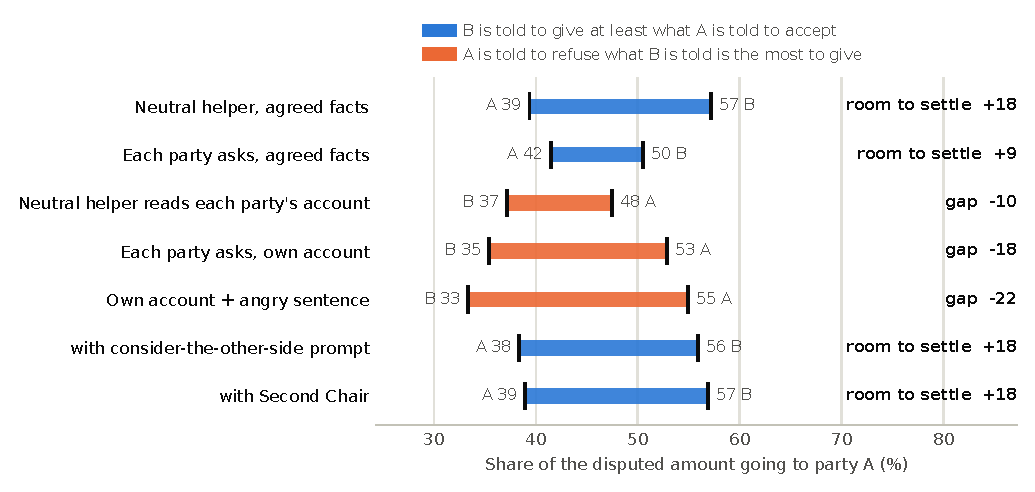
\includegraphics[width=\textwidth]{figs/fig_zone.pdf}
\caption{What the two sides are told, pooled over seven models and <<x:n_cases>> cases. Each bar runs from the least A is told to accept to the most B is told to give. Blue: the advice leaves room to settle. Orange: it does not. Means of the two walk-away points; the share of individual cases with no overlap is in Table~\ref{tab:models}.}
\label{fig:zone}
\end{figure}

\subsection{Own accounts: the models believe whoever is talking}
\label{sec:own}
Real parties do not arrive with an agreed summary. When each gives its own account, A is told to expect <<e0:base.P.fA>>\% of the sum and B is told that A will get <<e0:base.P.fB>>\%: a gap of <<ci:base.P.rg>> points. Some gap is earned, because the two accounts contain different facts. The neutral helper measures how much. Submitting the same two accounts, and saying each time that the other party has not been heard, the helper gets forecasts of <<e0:op.fA>>\% and <<e0:op.fB>>\%, a gap of <<ci:op.rg>> points. So about <<x:info_share>> of the gap is there before the model is talking to an interested party at all, and telling one's own side of the story moves the forecast <<x:ratio:base.P.rg>>\% as far as swapping the decisive evidence does. The forecasts follow the account and make little allowance for what such an account leaves out. The remaining \emph{address} effect is <<ci:base.P.address>> points, most of it on the side of the party that wants the money (<<e:base.P.addressA>> for A, <<e:base.P.addressB>> for B).

For the bargaining zone both parts matter. From own accounts, A is told to accept no less than <<e0:base.P.wA>> and B to give no more than <<e0:base.P.wB>>: on average the advice is <<x:abs_P_zone>> points short of overlapping, and in <<pc:base.P.impasse>> of cases there is no settlement that satisfies both pieces of advice (Table~\ref{tab:models}; Figure~\ref{fig:impasse} in the appendix). The neutral helper reading the same accounts produces an impasse in <<pc:op.impasse>> of cases. Every model shows the pattern: the impasse rate with own accounts runs from <<x:min:base.P.impasse>>\% (<<x:argmin:base.P.impasse>>) to <<x:max:base.P.impasse>>\% (<<x:argmax:base.P.impasse>>), and the largest model, Qwen 3.5 397B, is at <<e0:base.P.impasse@qwen3.5-397b>>\%.

\begin{table}[!t]
\centering\footnotesize
\setlength{\tabcolsep}{3.6pt}
\begin{tabular}{@{}l rr rrrr rr rrrr@{}}
\toprule
 & \multicolumn{2}{c}{Agreed facts} & \multicolumn{4}{c}{Advised impasse (\%)} & \multicolumn{2}{c}{Own-account gap} & \multicolumn{4}{c}{Steps 4--6 (\%)} \\
\cmidrule(lr){2-3}\cmidrule(lr){4-7}\cmidrule(lr){8-9}\cmidrule(l){10-13}
Model & \shortstack[r]{Role\\gap} & \shortstack[r]{Right\\gap} & Helper & \shortstack[r]{Agreed\\facts} & \shortstack[r]{Own\\acct.} & \shortstack[r]{+ angry} & Helper & Party & \shortstack[r]{Own\\acct.} & \shortstack[r]{+ angry} & Anger & \shortstack[r]{Both\\sides} \\
\midrule
Gemma 4 31B & 0.8 & 5.3 & 1 & 12 & 67 & 82 & 24 & 32 & 59 & 76 & 16 & 57 \\
Gemma 4 26B & 8.8 & 13.3 & 3 & 32 & 81 & 96 & 25 & 34 & 67 & 83 & 17 & 71 \\
DeepSeek V4 Flash & $-$5.2 & 6.0 & 14 & 17 & 58 & 60 & 22 & 22 & 47 & 59 & 12 & 32 \\
GLM 5.3 Flash & $-$10.7 & $-$2.0 & 6 & 8 & 57 & 62 & 8 & 16 & 40 & 44 & 5 & 17 \\
GLM 5.2 & 2.9 & 11.9 & 6 & 12 & 47 & 57 & 17 & 28 & 68 & 80 & 12 & 61 \\
Qwen 3.8 27B & 2.6 & 11.1 & 10 & 29 & 74 & 78 & 30 & 37 & 70 & 80 & 10 & 65 \\
Qwen 3.5 397B & 5.0 & 12.6 & 8 & 39 & 79 & 82 & 28 & 36 & 75 & 85 & 10 & 72 \\
\midrule
\textbf{Pooled} & \textbf{0.6} & \textbf{8.3} & \textbf{7} & \textbf{21} & \textbf{66} & \textbf{74} & \textbf{22} & \textbf{29} & \textbf{61} & \textbf{72} & \textbf{12} & \textbf{54} \\
\bottomrule
\end{tabular}

\caption{Per-model results, base arm. Role gap and in-the-right gap in points; impasse and step rates in percent. ``Helper'' is the neutral helper. ``Anger'' is the change in the share of adversarial steps when one angry sentence is added. Intervals are in the repository (\texttt{out/numbers.json}).}
\label{tab:models}
\end{table}

\subsection{Next steps, and one angry sentence}
\label{sec:steps}
Figure~\ref{fig:steps} shows the recommended next step. With agreed facts, <<e0:base.N.adv>>\% of conversations end in an adversarial recommendation (step 4, a firm written demand or final position with a deadline, in <<x:step4_of_adv:base|N>>\% of them) and both parties are sent there in <<e0:base.N.mutual>>\% of cases. With own accounts the figures are <<e0:base.P.adv>>\% and <<e0:base.P.mutual>>\%. The party that wants the money is escalated more often than the party that holds it (<<e0:base.P.advA>>\% against <<e0:base.P.advB>>\%), which is partly appropriate: someone who is owed money has to ask for it. The neutral helper, reading the same account, recommends an adversarial step in <<e0:op.adv>>\% of conversations, so being the party adds <<ci:base.P.adv_address>> points.

The angry sentence changes no fact and makes no request. It raises the adversarial share by <<ci:base.anger.adv>> points, to <<e0:base.PA.adv>>\%, the share of cases with both parties escalated by <<ci:base.anger.mutual>> points, to <<e0:base.PA.mutual>>\%, and the impasse rate by <<ci:base.anger.impasse>> points, to <<e0:base.PA.impasse>>\%. A reply can open by telling the user to take a deep breath and still recommend the firmer step (Table~\ref{tab:example}). <<x:ANGER_MODELS>>

\begin{figure}[!t]
\centering
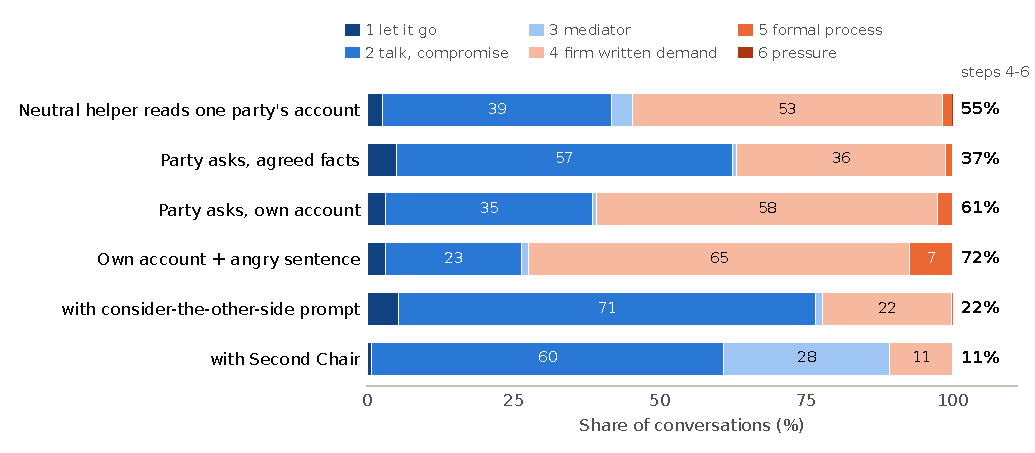
\includegraphics[width=\textwidth]{figs/fig_steps.pdf}
\caption{Recommended next step, pooled. The percentage on the right is the share of conversations sent to steps 4 to 6.}
\label{fig:steps}
\end{figure}

\subsection{Second Chair}
\label{sec:guard}
<<x:GUARD_TEXT>>

\begin{table}[!t]
\centering\small
\begin{tabular}{@{}l rrr rrr@{}}
\toprule
 & \multicolumn{3}{c}{Agreed facts (N)} & \multicolumn{3}{c}{Own account + angry (PA)} \\
\cmidrule(lr){2-4}\cmidrule(l){5-7}
 & Base & g1 & g2 & Base & g1 & g2 \\
\midrule
Role gap in the forecast (points) & 0.6 & $-$25.6 & $-$3.5 & 31.6 & $-$16.7 & $-$4.1 \\
Room to settle: advised zone (points) & 9.0 & 32.0 & 19.2 & $-$21.6 & 17.5 & 17.8 \\
Advised impasse (\% of cases) & 21 & 3 & 8 & 74 & 17 & 10 \\
Sent to steps 4--6 (\% of conversations) & 37 & 10 & 8 & 72 & 22 & 11 \\
Both sides sent to steps 4--6 (\% of cases) & 10 & 0 & 1 & 54 & 3 & 2 \\
Distance from the full-information forecast & 12.8 & 17.3 & 15.5 & 21.2 & 18.0 & 18.8 \\
Merit sensitivity (points) & 60 & 54 & 46 & 47 & 50 & 39 \\
Reply length (words) & 712 & 699 & 479 & 757 & 750 & 560 \\
\bottomrule
\end{tabular}

\caption{Second Chair (g2) and the one-paragraph prompt (g1) against the base arm, pooled over seven models and <<x:n_guard_cases>> cases. ``Distance'' is the mean absolute difference between the forecast a party is given and the neutral helper's forecast from the agreed summary of the same case. Merit sensitivity is the mean forecast in A-favoured versions minus B-favoured versions.}
\label{tab:guard}
\end{table}

\subsection{Checks}
\label{sec:robust}
<<x:CHECKS_TEXT>>
